\section{Introduction}

eBPF is now on the performance-critical paths of production systems: the Kubernetes networking datapath (Cilium~\cite{cilium}), Meta's layer-4 load balancer (Katran~\cite{katran}), fleet-wide observability and profiling (BCC~\cite{bcc}), runtime security monitoring (Tracee~\cite{tracee}), and CPU scheduling (\texttt{sched\_ext}~\cite{sched_ext_lwn}).  These programs execute on every packet, system call, or scheduling event, so each nanosecond of per-event cost is multiplied across a fleet.  eBPF's safety comes from an in-kernel compilation pipeline: a userspace compiler lowers each program to bytecode, the kernel verifier proves memory safety and termination~\cite{gershuni2019simple}, and a deliberately simple just-in-time compiler (JIT) translates the verified bytecode to native code one instruction at a time.

\textbf{eBPF users pay for verified safety with performance, and the loss cannot be recovered by rewriting bytecode alone.}  Our characterization over 54 microbenchmarks extracted from production eBPF programs shows the same C code runs up to twice as slow through the eBPF pipeline as when compiled directly to native code (1.57$\times$ geomean on x86-64; Figure~\ref{fig:gap}).  The gap is structural.  The single-pass kernel JIT cannot recognize multi-instruction patterns: a 64-bit variable rotate---one \texttt{ROL} instruction natively---arrives at the JIT as eight bytecode instructions and leaves as 15 machine instructions.  Fixing the JIT in place is unattractive: any change needs upstream acceptance and a long release cycle, enlarges the trusted computing base (TCB) that years of formal-methods work have hardened~\cite{nelson2020specification,vishwanathan2023verifying}, and grows per-architecture kernel code.  Moreover, the pipeline decides everything at load time, before deployment-time facts---stable map contents, biased branches---are visible.

\begin{figure}[t]
\begin{minipage}[t]{0.48\linewidth}
\centering
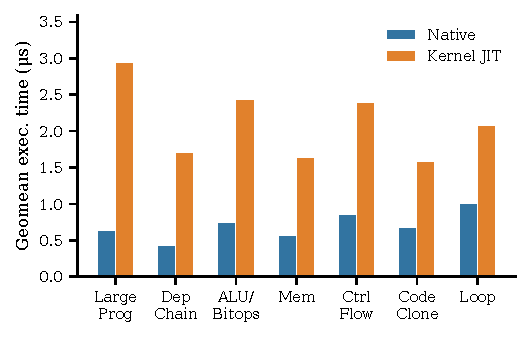
\includegraphics[width=\linewidth]{figs/sec-3-perf-gap-fig.pdf}
\caption{Kernel-JIT eBPF vs.\ native code (LLVM \texttt{-O2}) by benchmark category: the same C code runs up to 2$\times$ slower.}
\label{fig:gap}
\end{minipage}\hfill
\begin{minipage}[t]{0.48\linewidth}
\centering
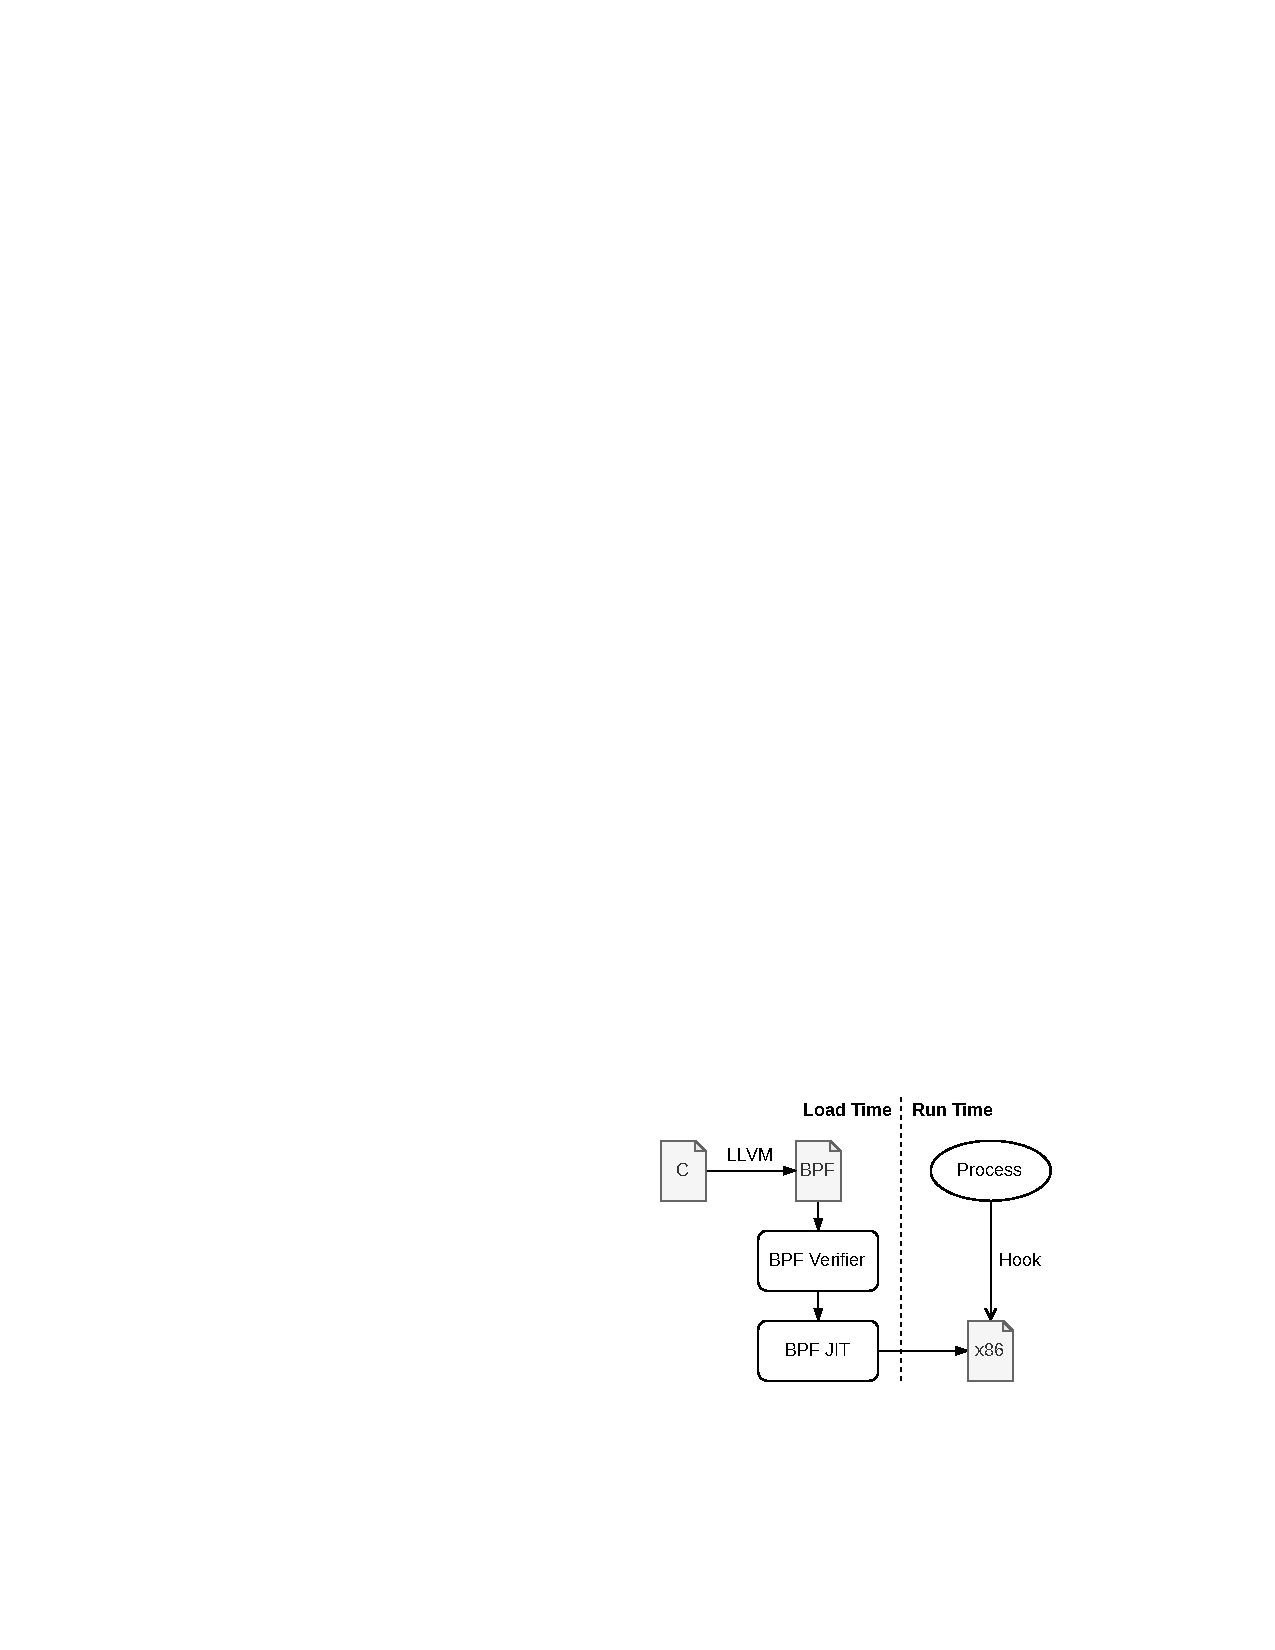
\includegraphics[width=\linewidth]{figs/sec-4-pipeline-fig.pdf}
\caption{Kops: each operation carries a \emph{proof sequence} the stock verifier checks and a \emph{native emit} the JIT compiles; Lean~4 proves them equivalent.}
\label{fig:kops}
\end{minipage}
\end{figure}

\noindent\textbf{Related Work:} Existing eBPF optimizers---K2's synthesis~\cite{xu2021synthesizing}, Merlin~\cite{mao2024merlin}, and EPSO~\cite{zhu2025epso}---rewrite programs \emph{within} the instruction set before load, so they inherit its expressiveness ceiling and see no deployment workload.  EPASS (a 2025 eBPF Foundation project~\cite{huang2025epass}) transforms programs at load time for programmability and safety within the ISA; we complementarily target the performance gap \emph{below} the ISA and \emph{after} deployment.  Jitterbug~\cite{nelson2020specification} and Agni~\cite{vishwanathan2023verifying} formally verify the existing JIT and verifier but do not extend the pipeline; we adopt the same philosophy by proving new operations equivalent to verifier-checked bytecode.  Rust-based extensions~\cite{jia2025rex} trade independent load-time checking for toolchain trust, and profile-guided optimization is standard for userspace binaries (BOLT~\cite{panchenko2019bolt}) but has no counterpart for deployed eBPF programs.

\section{Closing the Gap, Below the ISA and After Deployment}

The goal of this project is to \textbf{make verified eBPF programs performance-competitive with native code while the stock kernel verifier remains the sole safety authority}: every optimized program is re-checked by the unmodified verifier before it runs, so no optimizer ever joins the safety argument.  We attack the gap at the two points the current pipeline cannot reach.

\noindent\textbf{Below the ISA --- Kops.}  Kops~\cite{zheng2026kops} is an extension interface through which kernel modules add new operations to the pipeline without modifying the kernel core (Figure~\ref{fig:kops}).  Each operation carries two forms: a \emph{proof sequence} of vanilla eBPF instructions that the existing verifier checks on every load, and a \emph{native emit} of machine instructions that the JIT compiles.  A compile-time recognizer rewrites programs to use the operations; because the verifier checks the proof sequence, neither the recognizer nor the sequence joins the TCB---the native emit is the only per-operation addition, and we discharge that trust with Lean~4 proofs that the emit computes the same result as its proof sequence.

\noindent\textbf{After deployment --- BpfReJIT.}  BpfReJIT re-optimizes deployed programs using facts visible only at runtime.  An in-process shim intercepts an \emph{unmodified} application's \texttt{BPF\_PROG\_LOAD} and attachment calls; a pass engine rewrites raw bytecode using runtime side inputs (captured map contents, per-site PMU branch profiles); and the shim resubmits every candidate through the stock verifier and JIT, so a rejected candidate simply leaves the original program running.  The same boundary supports load-time specialization and in-place replacement of running programs via existing kernel APIs.

\noindent\textbf{Measurement substrate --- an open benchmark.}  Both mechanisms are evaluated on our benchmark built from six production applications (Cilium, Katran, Tracee, Tetragon, BCC, and an eBPF continuous profiler): 146 eBPF programs, 42 microbenchmarks, real workloads, hidden correctness checks that detect unsound transformations, and automated x86-64/ARM64 runs on stock kernels.

\noindent\textbf{Preliminary Results:} Kops with seven hardware-idiom operations (rotate, conditional select, bit extract, etc.) speeds up microbenchmarks by up to 24\% on x86-64 and 22\% on ARM64---recovering 42\% of the gap to native code---improves Cilium and Katran datapath throughput by up to 12\%, and shrinks generated native code by 12--23\%, with no measurable load-time overhead~\cite{zheng2026kops}.  BpfReJIT transparently applies load-time plans to all six unmodified applications on stock kernels.  An upper-bound study using the same interface to load whole-program native replacements reaches 2.358$\times$ on Cilium---quantifying the remaining reward---while our LLM-agent exploration harness has discovered optimizations of up to 34\% on suite programs.  The benchmark is open sourced at \url{https://github.com/eunomia-bpf/bpf-bench}.

\noindent\textbf{Tasks:} Preliminary results expose profitability, not mechanism, as the open problem: applying every matched Kops site can regress (0.995$\times$ on Katran under a coverage-maximizing policy), and a profile-guided branch-layout pass improved one complete six-application run but regressed a rerun.  We will therefore pursue: \textbf{Task 1:} a cost-model-guided per-site profitability policy for Kops, replacing coverage maximization.  \textbf{Task 2:} extend the operation set beyond hardware idioms to the map- and helper-adjacent patterns that dominate real datapaths, where idioms alone recover only 5.4\% of the achievable gap on Cilium.  \textbf{Task 3:} stability-aware gating for profile-guided re-optimization, validated on held-out runs.  \textbf{Task 4:} complete and evaluate live replacement of running programs across links, perf events, tracepoints, XDP, and tail-call program arrays, with phase-change recovery that reverts expired specializations.  \textbf{Task 5:} release the benchmark suite and characterization, and engage upstream through a kernel RFC for the Kops interface.

\section{Milestones and Expected Outcomes}

\noindent September 1, 2026 --- Project start.\\
\textbf{Milestone 1:} December 1, 2026 --- (Tasks 1, 5) Kops profitability policy evaluated on all six applications; benchmark suite v1.0 release. 1st update blog post.\\
\textbf{Milestone 2:} May 1, 2027 --- (Tasks 2, 3) extended operation set; gated profile-guided passes validated on held-out runs. 2nd progress update.\\
\textbf{Milestone 3:} August 1, 2027 --- (Task 4) live-replacement coverage and phase-change recovery evaluation; upstream RFC posted. 2nd blog post.

The expected outcomes are open-source releases of the benchmark suite, the Kops kernel modules with their Lean~4 proofs, and the BpfReJIT framework, all usable on stock kernels; at least two blog posts; papers at top systems venues (OSDI/SOSP); and an upstream conversation on extending the eBPF pipeline with verified native operations.  The PI and her graduate student are well positioned for this research through their expertise in extending eBPF to new domains~\cite{zheng2025extending,yang2025egpu} and building novel systems-debugging tools~\cite{Quinn_2022_omnitable}.
